\documentclass{standalone}
\usepackage{amsmath}
\usepackage[dvipsnames]{xcolor}
\usepackage{tikz} 
\usetikzlibrary{arrows, decorations.markings,decorations.pathreplacing,angles,quotes}
\usepackage{microtype}
\usepackage{fourier}

\definecolor{py_blue}{rgb}{0.12156862745098039, 0.4666666666666667, 0.7058823529411765}
\definecolor{py_orange}{rgb}{1.0, 0.4980392156862745, 0.054901960784313725}
\definecolor{py_green}{rgb}{0.17254901960784313, 0.6274509803921569, 0.17254901960784313}
\definecolor{py_red}{rgb}{0.8392156862745098, 0.15294117647058825, 0.1568627450980392}
\definecolor{py_purple}{rgb}{0.5803921568627451, 0.403921568627451, 0.7411764705882353}

\begin{document}

\begin{tikzpicture}
	\node[anchor=south west,inner sep=0] (Bild) at (0,0) {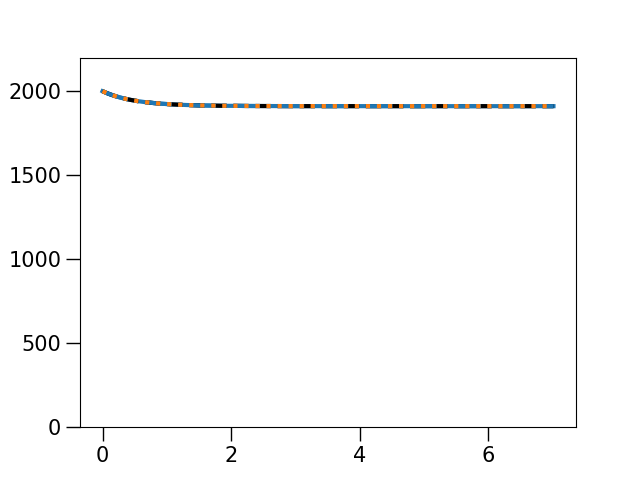
\includegraphics[scale=0.39]{low_c_blank}};
   		\begin{scope}[x=(Bild.south east),y=(Bild.north west)]
   			\node (Bild2) at ([xshift=2.75cm]Bild.east) {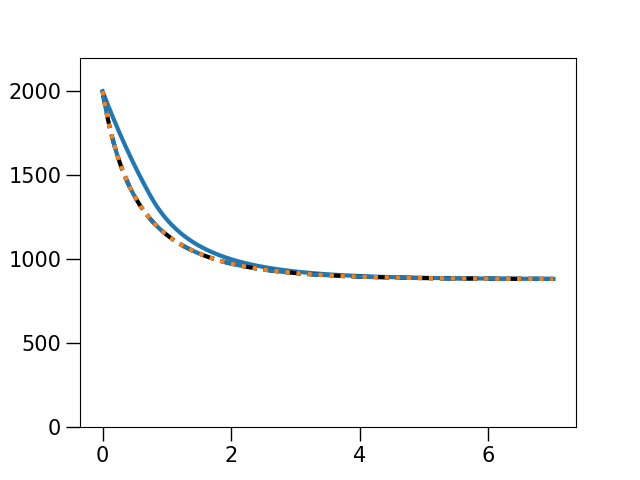
\includegraphics[scale=0.39]{inter_c_blank}};
   			\node (B3) at ([xshift=2.75cm]Bild2.east) {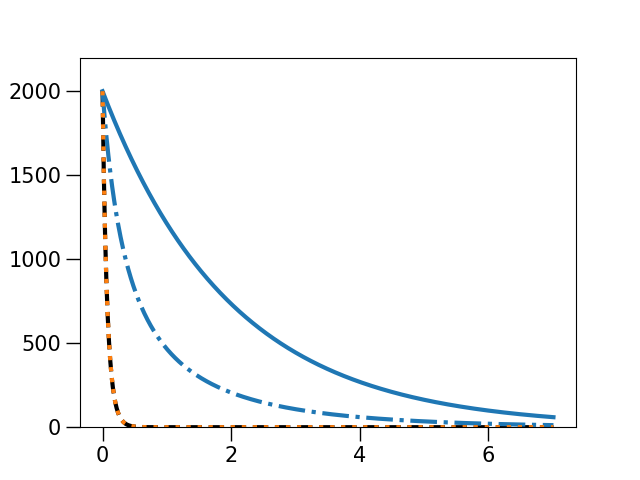
\includegraphics[scale=.39]{high_c_blank}};
        	\node at (Bild2.south) {time $t$ in days};
        	\node[rotate=90] at ([xshift=-.15cm]Bild.west) {population size};
        	\node at ([yshift=-.2cm]Bild.north) {$c=0.001$};
        	\node at ([yshift=-.3cm]Bild2.north) {$c=0.01$};
        	\node at ([yshift=-.3cm]B3.north) {$c=0.1$};
        	
			\draw[thick,color=py_blue] (1.25,0.8) -- node[right=5pt] {\small \color{black} biostatic + birth comp} (1.32,0.8);   
			\draw[thick,color=py_blue,dash dot] (1.25,0.72) -- node[right=5pt] {\small \color{black} biostatic + death comp} (1.32,0.72);        	
			\draw[thick,color=black,dashed] (1.25,0.64) -- node[right=6pt] {\small \color{black} biocidal + birth comp} (1.31,0.64);   
			\draw[thick,color=py_orange,dotted] (1.25,0.56) -- node[right=5pt] {\small \color{black} biocidal + death comp} (1.32,0.56);  
 			
    	\end{scope}
\end{tikzpicture}

\end{document}